\documentclass[../main_proj3.tex]{subfiles}

\graphicspath{{\subfix{Figures/}}}

\begin{document}

\subsection{Verification of code functionality}

Figure \ref{fig:single_z} shows the z coordinate of particle 1 for a simulation using the RK4 method over a simulation time of 50 microseconds. There is a clear oscillation as expected given that this solution should simulate the benchmark solution for which had the specific solution of equation \eqref{eq:specific_solution-eq_of_motion_z}. Since $z_0=20$ the amplitude of the oscillation is also 20. Further the expected period is decided by $\frac{2\pi}{\omega_z} = \frac{2\pi}{\sqrt{2qV_0/md^{2}}} \approx  9.1$ which is also period shown in the figure.

\begin{figure}[h!]
    \centering
    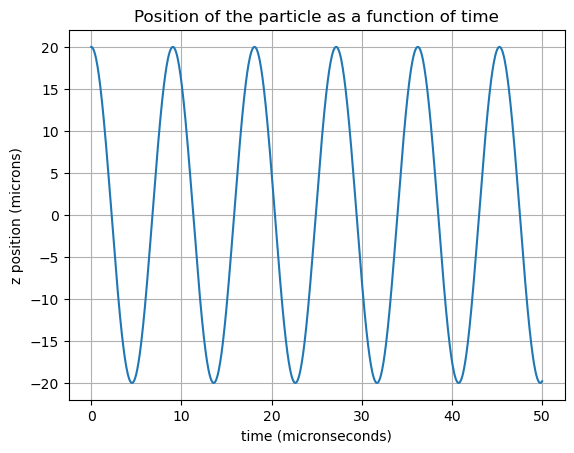
\includegraphics[width=0.9\linewidth]{Project 3/figures/single_particle_z_position.png}
    \caption{The z coordinate over time for a single particle in the Penning trap.}
    \label{fig:single_z}
\end{figure}
\begin{figure*}[ht]
    \centering
    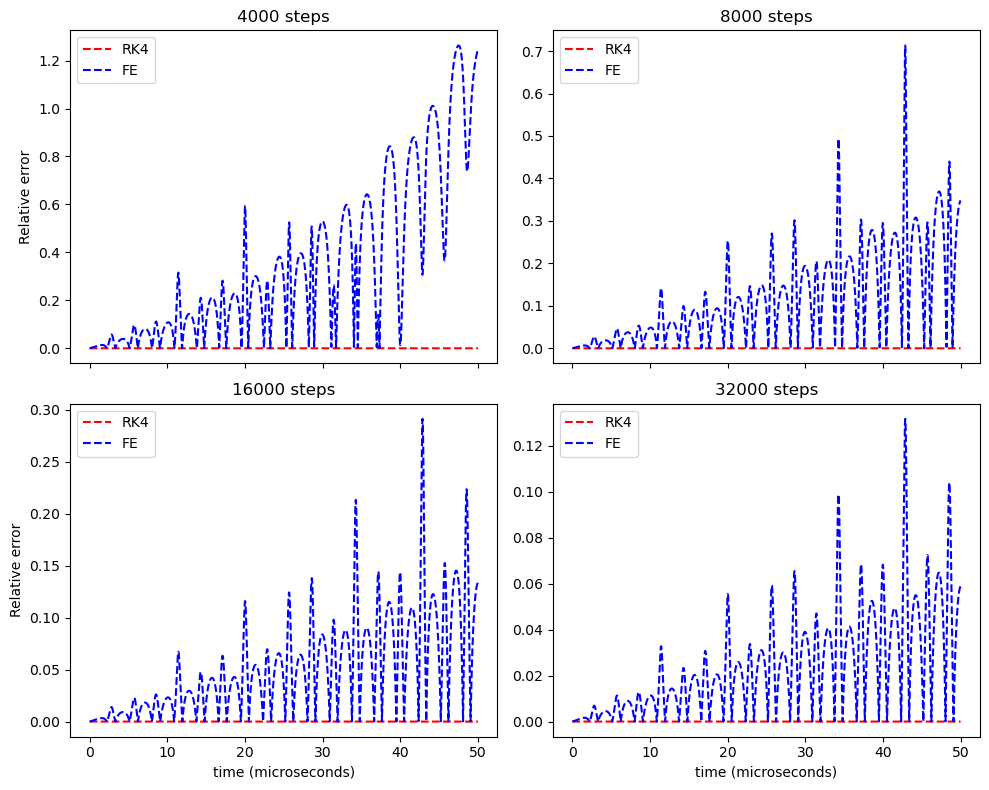
\includegraphics[width=.9\textwidth]{Project 3/figures/single_particle_relative_error.png} % Replace with your image file
    \caption{The relative error of the simulations method relative to the benchmark simulation.}
    \label{fig:rel_error}
\end{figure*}
To estimate the numerical accuracy of the simulation we benchmark the numerical simulation against the specific analytical solution. The relative error of simulating a single particle as a function of time is shown in Figure \ref{fig:rel_error}. The Figure shows how the relative error of FE decreases as expected when the number of steps increases. FE shows large improvements as $h$ is decreased; from relative errors larger then 1 (i.e. either two times as large values or different sign) to relative errors bellow 0.15 for 32000 steps on 50 microseconds. Based on the same numbers as in the plot the estimated error convergence rate for FE method is $1.4463$. For RK4 relative error is very small and already when the number of steps are 4000, this yields a error convergence rate of $2.4299$. The key point of the plot is that RK4 is a much more stable algorithm compared to FE, which is also in accordance with the theoretical global truncation error number of $\mathcal{O}(h^{4})$ and $\mathcal{O}(h)$ respectively.  



The position vector at the end of simulation for $n_{\text{steps}}=32000$ with RK4 is $\mathbf{r}(50) = \langle 21.7613,	38.9772, -19.8049 \rangle$ which is exactly the same as the analytical solution for the same particle. For lower amounts of steps the trend is that the radial plane is harder to simulate then the z-plane. This is likely due to the more complicated oscillations found in radially (see Figure \ref{fig:radial_plane_position}) then in the z-plane (see Figure \ref{fig:single_z}). 

Figure \ref{fig:radial_plane_position} shows the position of particle 1 and 2 in the radial plane. The left hand side plot shows the trajectories when the particles are not interacting. They follow a pattern of two different oscillations, as expected since there are multiple frequencies in the specific solution for a single particle. In the left hand side the trajectories are shown with particle interactions. Since the particles are equally charged we observe a repulsion of the particle trajectories towards the end. Further we allso observe who the regular oscillations of the left hand side plot are disrupted as a result of introducing the Coloumb force to the Lorentz force expression. 

\begin{figure*}[h]
    \centering
    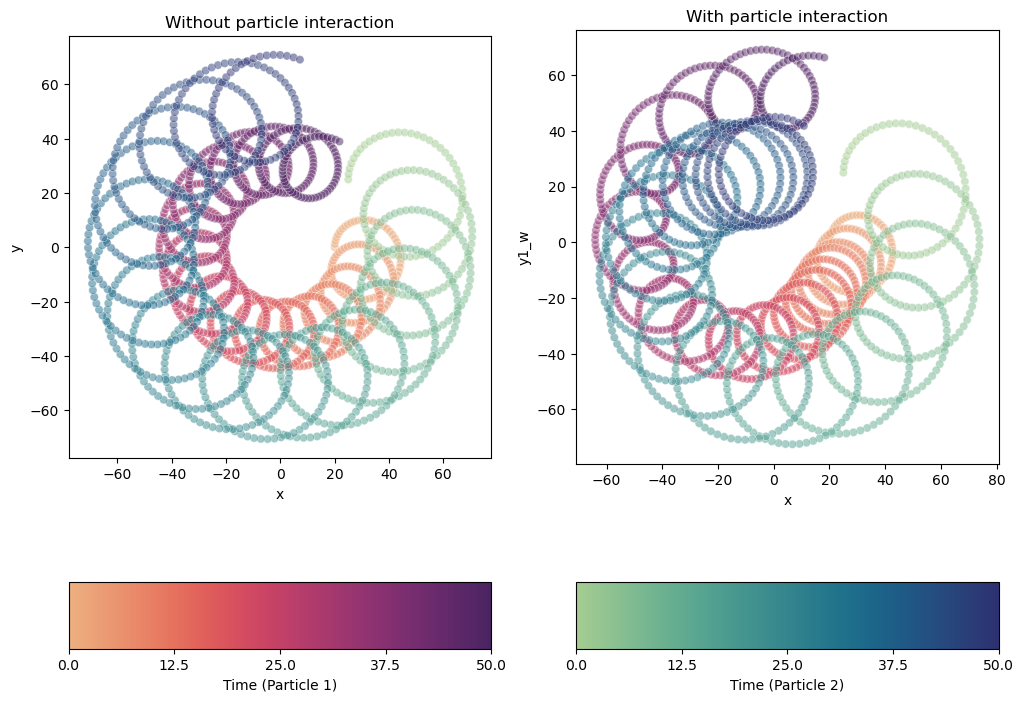
\includegraphics[width=.9\linewidth]{Project 3/figures/two_particles_xy_plane.png}
    \caption{The radial plane position as a function of time. The individual trajectories for particle 1 and 2 are colored in distinct color maps dependent on time in simulation.}
    \label{fig:radial_plane_position}
\end{figure*}

To further illustrate the interactions I refer to the Figure \ref{fig:phase-space} and \ref{fig:two_particles_3d} in the Appendix. In Figure \ref{fig:phase-space} the phase-space plots for the x and y-plane are shown. Based on visual analysis it seems that the velocities are altered (i.e. increased for particle 1 and decreased for particle 2 based on amplitude changes for the velocities) when Coloumb interactions are included. This is also reflected in Figure \ref{fig:radial_plane_position} where the trajectories for particle 1 are more stretched in the later part of the simulation while the trajectory of particle 2 is more condensed. From a physical point of it does make sense that energy can be transfered between the particles as the kinetic energy of particle 2 is higher then that of particle 1 given their initial velocities. In figure \ref{fig:two_particles_3d} the particle position is shown in 3d. More then anything else this plots illustrates both the osicllatory motion in the z- plane from figure \ref{fig:single_z} and the two phases shown in Figure \ref{fig:radial_plane_position}. 


\subsection{Resonance frequencies}

To explore of there are resonance phenomena in the Penning trap we simulated 100 particles with and without interactions with a time dependent electric field. Figure \ref{fig:100_full_omega_v} show the fraction of particles that remained in the trap after 500 microseconds of simulation as a function of the angular frequency $\omega_v$ (note the inverse y-axis). In the figure we observe some frequencies are more effective of pushing particles out of the trap, indicating that there are indeed some resonance phenomena present in the Penning trap. Thinking back to the benchmark simulation setup the particles have periodic trajectories whose period is dictated by the $\omega_+, \omega_-$ and $\omega_z$. Qualitatively this may be among the frequencies that should be avoided for $\omega_v$ as they might resonate? To conclude on this a more in depth simmulation and investigation. 

\begin{figure}[h!]
    \centering
    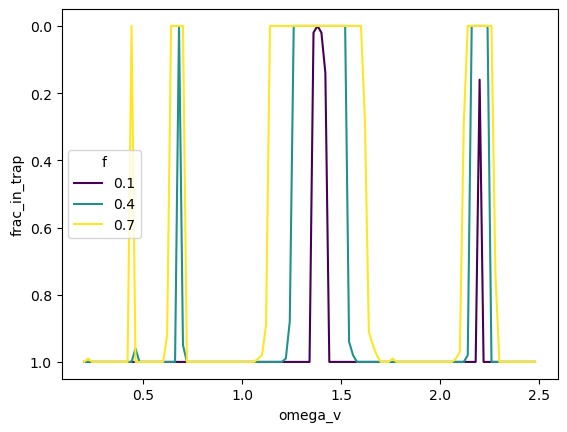
\includegraphics[width=0.9\linewidth]{Project 3/figures/100_particle_full_fq.png}
    \caption{The fraction of particles in the Penning trap after 500 microseconds of simulation as a function of the angular frequency $\omega_v$. The Note the inverse y axis.}
    \label{fig:100_full_omega_v}
\end{figure}

The amplitude $f$ of the oscillation of $V_0(t)$ around $V_0$ works to broaden the frequency intervals where the resonance occur. Mathematically this makes sense: An increase in $f$ will directly alter the the magnitude of $V_0(t)_{max}$. From the stability requirement shown in equation \eqref{eq:frequency_constraint} we know that an increase in $V_0$ will reduce the ratio on the LHS and thus making the Penning trap configuration less stable. 

The simulations in Figure \ref{fig:100_full_omega_v} are conducted without Coulomb interactions between the particles to reduce the computational cost. To investiagate the effect of Coloumb interactions we simulate the area $\omega_v \in(.64, .74)$ MHz with smaller steps of $.005$ MHz between values and with $f=.4$. Results are shown Figure \ref{fig:100_small_omega_v} where the dotted line shows the simulations with Coloumb interactions while the solid line is without as in Figure \ref{fig:100_full_omega_v}. The plot indicates that including particle interactions will broaden the intervals for which resonance occour. 

\begin{figure}[h!]
    \centering
    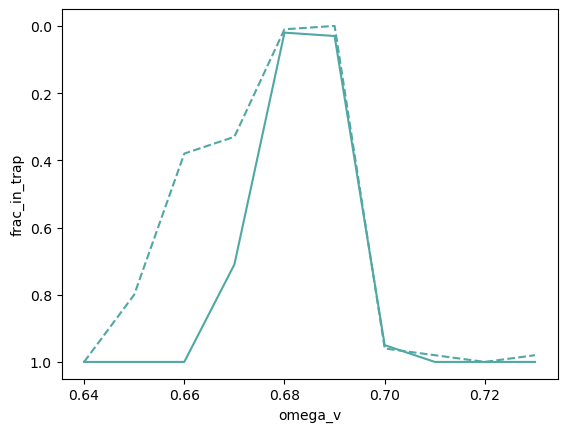
\includegraphics[width=0.9\linewidth]{Project 3/figures/100_particle_small_fq.png}
    \caption{The fraction of particles in the Penning trap after 500 microseconds of simulation as a function of the angular frequency $\omega_v$. The dotted line shows the simulation with interacting particles. The Note the inverse y axis.}
    \label{fig:100_small_omega_v}
\end{figure}


Note that for the investigation of resonace frequencies the initial values are randomly generated. When looking into the results I discovered that the seed was not set properly which will make results less trustworthy. However a larger issue is the sample size of 100 particles per $f, \omega_v$ configuration. This is a small number of particles and it is not likely that the we will approach convergence towards the ground truth. Despite this, I believe that the tendencies for the Penning trap to have resonance frequencies are illustrated due to the distinct changes in domain between frequencies. In addition we also observe that the favorable $\omega_v$ values are the same 
between $f$ values. 

\end{document}